% ============================================================
% EvidenceFirst submission source.
% Compile with pdflatex -> bibtex -> pdflatex -> pdflatex.
% ============================================================
\documentclass[runningheads,a4paper]{llncs}

\usepackage[T1]{fontenc}
\usepackage{amsmath,amssymb}
\usepackage{array}
\usepackage{booktabs}
\usepackage{graphicx}
\usepackage{multirow}
\usepackage{xcolor}
\usepackage{xspace}
\usepackage{pifont}
\usepackage{microtype}
\usepackage{tikz}
\usetikzlibrary{arrows.meta,positioning,calc,fit,backgrounds}

\setlength{\textfloatsep}{5pt plus 1pt minus 1pt}
\setlength{\floatsep}{4pt plus 1pt minus 1pt}
\setlength{\intextsep}{4pt plus 1pt minus 1pt}
\setlength{\abovecaptionskip}{3pt}
\setlength{\belowcaptionskip}{2pt}

\newcommand{\sys}{\textsc{EvidenceFirst}\xspace}
\newcommand{\eg}{\emph{e.g.},\xspace}
\newcommand{\ie}{\emph{i.e.},\xspace}
\newcommand{\calG}{\mathcal{G}}
\newcommand{\calP}{\mathcal{P}}
\newcommand{\calE}{\mathcal{E}}
\newcommand{\calT}{\mathcal{T}}

\begin{document}

\title{\sys: Evidence-State Monitoring for Auditable GraphRAG Systems}
\titlerunning{\sys for Web GraphRAG Monitoring}

\author{Anonymous Author(s)}
\authorrunning{Anonymous}
\institute{
  Institution anonymized for review\\
  \email{email@anonymized.com}
}

\maketitle

% ============================================================
\begin{abstract}
% ============================================================

Fixed-context Web GraphRAG systems combine Web pages, graphs, and LLM readers,
but operators still need to know which evidence condition preceded a suspicious
answer. \sys is an evidence-state monitoring and auditing framework
for GraphRAG systems. Before generation, a deterministic checker assigns each
question to a checked candidate path, repaired path, residual graph gap, or
passage-fallback state; the saved state records the repair or fallback route,
reader evidence, selector decision, and audit fields. The objective is
evidence-state analysis rather than leaderboard optimization. Across
HotpotQA-1000 and 2WikiMultiHopQA-500, \sys remains within the operating range
of recent GraphRAG baselines while exposing audit-risk queues that can be
replayed without regeneration. Empirically, saved audit signals form review
queues whose top-20\% strata reach 67.0\% and 40.0\% error rates on HotpotQA and
2Wiki; adding graph-state fields to answer-selection signals improves
error-detection AUC (0.6077$\rightarrow$0.6321 on HotpotQA) and, more
importantly, supplies typed routing causes: inside selection-conditioned queues,
selected unrepaired-incomplete Hotpot cases and non-selected residual-gap 2Wiki
cases are 26.6 and 33.3 error points worse than their respective comparison
strata. Rather than
predicting why a GraphRAG system failed, \sys records a replayable
evidence-state trace that helps failures be routed, audited, and recomputed
after deployment.

\keywords{Knowledge Graphs \and RAG on the Web \and GraphRAG \and
Evidence Observability \and Auditing \and Routing}
\end{abstract}

% ============================================================
\section{Introduction}
\label{sec:intro}
% ============================================================

\begin{center}
\vspace{-2pt}
\refstepcounter{figure}\label{fig:overview_taxonomy}
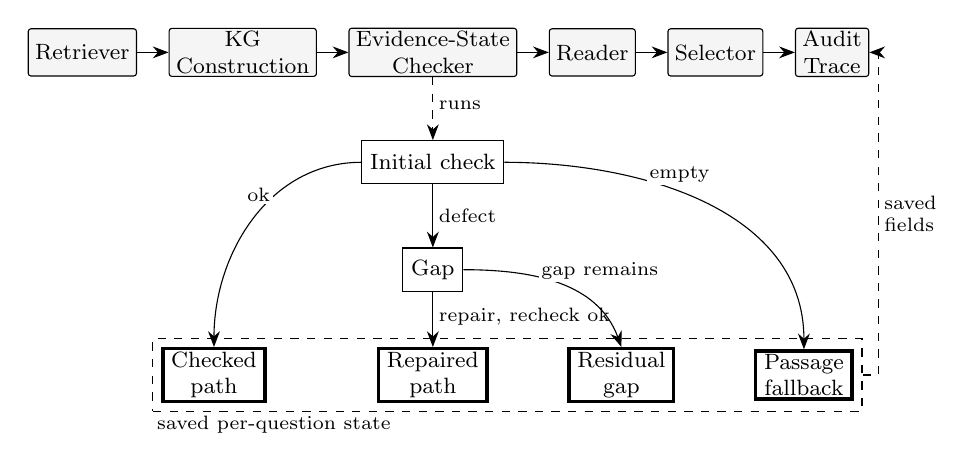
\begin{tikzpicture}[
  font=\footnotesize,
  >={Stealth[length=2mm]},
  mod/.style={draw, rounded corners=1pt, align=center, minimum height=6mm,
              inner xsep=2.5pt, inner ysep=1.2pt, fill=black!4},
  st/.style={draw, align=center, minimum height=5.5mm,
             inner xsep=3pt, inner ysep=1.2pt, fill=white},
  term/.style={st, very thick},
  lab/.style={font=\scriptsize, fill=white, inner sep=1pt},
  node distance=3mm and 4mm
]

% ---------- top: pipeline ----------
\node[mod] (ret)  {Retriever};
\node[mod, right=of ret]  (kgc) {KG\\Construction};
\node[mod, right=of kgc]  (chk) {Evidence-State\\Checker};
\node[mod, right=of chk]  (rdr) {Reader};
\node[mod, right=of rdr]  (sel) {Selector};
\node[mod, right=of sel]  (aud) {Audit\\Trace};

\draw[->] (ret) -- (kgc);
\draw[->] (kgc) -- (chk);
\draw[->] (chk) -- (rdr);
\draw[->] (rdr) -- (sel);
\draw[->] (sel) -- (aud);

% ---------- bottom: state machine ----------
\node[st, below=8mm of chk] (init) {Initial check};
\node[st, below=8mm of init] (gap) {Gap};

% terminal states row (below gap)
\node[term, below=7mm of gap]        (repaired) {Repaired\\path};
\node[term, left=14mm of repaired]   (checked)  {Checked\\path};
\node[term, right=10mm of repaired]  (residual) {Residual\\gap};
\node[term, right=10mm of residual]  (fall)     {Passage\\fallback};

% transitions
\draw[->] (init.west) to[out=180,in=90] node[lab, pos=0.4, above left=-2pt] {ok} (checked.north);
\draw[->] (init) -- node[lab, pos=0.5, right=1pt] {defect} (gap);
\draw[->] (init.east) to[out=0,in=90] node[lab, pos=0.35, above right=-2pt] {empty} (fall.north);
\draw[->] (gap) -- node[lab, pos=0.45, right=1pt] {repair, recheck ok} (repaired);
\draw[->] (gap.east) to[out=0,in=110] node[lab, pos=0.4, above right=-2pt] {gap remains} (residual.north);

% dashed link: checker runs the state machine
\draw[dashed,->] (chk.south) -- node[lab, right=1pt, pos=0.45] {runs} (init.north);

% dashed: terminal states saved to the audit trace
\begin{scope}[on background layer]
\node[draw, dashed, inner sep=3pt, fit=(checked)(repaired)(residual)(fall)] (states) {};
\end{scope}
\node[font=\scriptsize, anchor=north west, inner sep=1.5pt]
      at (states.south west) {saved per-question state};
\draw[dashed,->] (states.east) -- ++(2mm,0) |- node[lab, pos=0.25, right=1pt, align=left] {saved\\fields}
      (aud.east);

\end{tikzpicture}
\parbox{\linewidth}{\scriptsize\textbf{Fig.~\thefigure.}
Evidence-state pipeline and state-machine transitions. The Evidence-State
Checker runs a structural state machine whose terminal state is saved
per-question and written to the audit trace for replayable inspection.}
\vspace{-4pt}
\end{center}

GraphRAG research has mainly optimized retrieval, reasoning, and generation
over retrieved text and graph structure. In an enterprise search or public Web
QA service, however, the operational question after a bad answer is often not
``which model scored higher?'' but ``which evidence condition preceded this
case?'' For example, a Web QA service answering from search-result pages must,
after a complaint, determine whether the retrieved pages lacked a bridge entity,
the constructed graph was disconnected, or the reader misread connected evidence
-- distinctions invisible in answer-plus-context logs. The failure may come from
missing retrieved context, an incomplete graph,
an absent bridge entity, disconnected evidence, a reader mistake, or final
answer selection. RAG grounds language-model answers in retrieved
text~\cite{lewis2020rag}, while KG-RAG and GraphRAG systems add
entity-relation structure over retrieved corpora
~\cite{edge2024graphrag,guo2024lightrag,han2025graphragsurvey}. Yet most
systems expose only the final answer and retrieved context, leaving operators
without a stable evidence-state trace for routing and audit.

\sys treats the evidence graph as an observable state object before the reader
is called. The checker assigns each question to a checked candidate path,
repaired path, residual graph gap, or passage-fallback state. That state is
operational rather than merely logged: it selects graph repair or passage
fallback, constrains which evidence is passed to generation, records the
downstream selection decision, and can be replayed from saved artifacts.

The objective of this work is evidence-state analysis rather than leaderboard
optimization. We therefore evaluate on representative subsets that allow
detailed replay inspection and audit analysis. HotpotQA and 2Wiki provide
retrieved passages, entity mentions, and linked evidence graphs; \sys studies
how a GraphRAG system exposes and uses the retrieved graph state before
generation.

\paragraph{Contributions.}
This paper makes three contributions:
\begin{itemize}
    \item \textbf{Evidence-state abstraction.} We introduce a lightweight
    abstraction that ties each answer artifact to a checked, repaired,
    residual, or fallback graph state computed before generation.
    \item \textbf{Replayable audit protocol.} We support recomputation of
    reported claims, risk strata, path-state summaries, and evidence-visibility
    diagnostics from saved artifacts without regeneration.
    \item \textbf{Failure routing mechanism.} We study how graph-state signals
    facilitate repair and inspection workflows, separating graph repair,
    reader/selector inspection, and context review.
\end{itemize}

% ============================================================
\section{Related Work}
\label{sec:related}
% ============================================================

\paragraph{RAG, GraphRAG, and multi-hop retrieval.}
RAG conditions a language model on retrieved evidence~\cite{lewis2020rag}, while
GraphRAG systems organize evidence as entity, relation, or community structures
~\cite{edge2024graphrag,guo2024lightrag,han2025graphragsurvey}. Hierarchical,
memory-oriented, and reasoning-aware variants structure context as trees,
long-term memories, hybrid records, or iterative retrieval paths
~\cite{sarthi2024raptor,gutierrez2024hipporag,li2024structrag,trivedi2022ircot,arag2026,yu2025hoprag}.
These systems mainly acquire, traverse, or compress evidence for a reader. \sys
targets a later operational stage: after graph evidence is retrieved or
constructed, it records whether the graph is checked, repaired, residual, or
fallback before generation.

\paragraph{Observability and traceability in information systems.}
Information systems expose internal state for later inspection: databases
preserve transaction logs~\cite{mohan1992aries}, distributed systems expose
execution traces~\cite{sigelman2010dapper}, and data-management systems track
provenance or lineage~\cite{buneman2001why,cheney2009provenance}. GraphRAG
systems have an analogous need, but saved artifacts usually stop at retrieved
evidence, generated text, or tool-call logs. \sys imports this observability
perspective into Web GraphRAG by recording the graph condition that routed each
answer artifact.

\paragraph{Verification and auditability.}
RAG evaluation frameworks score retrieval, generation, and answer quality
~\cite{es2024ragas,saadfalcon2024ares,chen2024rgb,friel2024ragbench}, while
attribution studies ask whether claims are grounded in identifiable sources
~\cite{rashkin2023attribution,gao2023alce,wallat2024faithfulness}. S2G-RAG
emits text gap items~\cite{s2grag2026}, and RAGChecker defines diagnostic
metrics for retrieval and generation modules~\cite{ru2024ragchecker}. \sys
narrows the observable object to a per-question graph state stored before
generation, used for repair/fallback routing, and replayed from saved artifacts.

% ============================================================
\section{Method}
\label{sec:method}
% ============================================================

\subsection{Web Knowledge-RAG Problem Setting}

We model a Web GraphRAG query as fixed-context inference over retrieved or
provided Web evidence. Given a question $q$, candidate passages
$\calP=\{p_i\}$, and a per-question evidence graph $\calG=(V,E)$ built from the
same visible evidence, the system outputs a short answer $a$ and a diagnostic
record $D$. Nodes in $\calG$ are entities or evidence units, and edges are
extracted relations, support links, or passage-level associations. The setting
covers search results, Wikipedia-style pages, entity descriptions, and linked
Web documents; it does not assume live crawling or changing Web content during
inference.

\sys records a structural path-state contract before generation. The graph
state is one of four states: a checked candidate path, a repaired path after
localized graph expansion, a residual graph gap after unsuccessful repair, or a
passage-fallback state when usable graph evidence is absent. The diagnostic
record $D$ stores path-checked status, path length, gap type, missing-entity and
disconnected-pair counts, repair/fallback tags, and the final answer-selection
flag. The recorded state authorizes the repair, fallback, or evidence route that
generation receives.

\begin{table}[!htbp]
\centering
\caption{Evidence-state contract used by \sys. The states are operational
routing states over the retrieved graph.}
\label{tab:state_contract}
\scriptsize
\setlength{\tabcolsep}{2.4pt}
\resizebox{\linewidth}{!}{%
\begin{tabular}{p{2.5cm}p{4.2cm}p{4.1cm}p{3.8cm}}
\toprule
State & Entry condition & Operational route & Saved fields \\
\midrule
Checked path & Candidate path satisfies entity mapping, answer-type filter, and
minimum path length & Terminal reader route: pass extracted chain, with local
passages when enabled & \texttt{chain\_complete}, chain length, empty gap label \\
Repaired path & Initial gap triggers entity-augmentation or bridge repair and recheck becomes complete &
Transition from gap to terminal reader route; preserve repair provenance &
repair tags, \texttt{chain\_complete}, chain length \\
Residual gap & Recheck remains incomplete or short after repair & Terminal
reader route with available triples/passages and retained graph cause & gap
label, missing entities, disconnected-pair count, repair tags \\
Passage fallback & No usable triples or graph evidence is absent & Terminal
passage route; mark graph evidence unavailable & fallback tags, empty/unknown
chain fields \\
\bottomrule
\end{tabular}
}
\end{table}

\paragraph{Algorithmic contract.}
Given $q$, $\calP$, and $\calG$, \sys executes a fixed state machine before the
reader output. It extracts question entities, maps them to graph nodes by exact,
substring, and token-overlap matching, selects candidate answer nodes, filters
them by coarse answer type, and tests shortest paths in the evidence subgraph.
If an adequate path exists, the state is checked and the extracted chain is sent
to the reader. Otherwise, the checker emits \texttt{missing\_entities},
\texttt{disconnected}, \texttt{bridge}, or \texttt{short\_chain}; empty graph
evidence becomes passage fallback. Missing entities trigger entity-augmentation repair,
disconnected pairs trigger bridge repair over at most five endpoint pairs,
and every repair is followed by the same structural recheck. A complete recheck
becomes a repaired path; otherwise the residual or fallback state is retained
through generation and selection. These rules are fixed before evaluation and
use no gold answers or support facts at test time.

\subsection{Evidence-First Inference}

\sys performs inference by applying the same state contract to every question:
it builds or loads a per-question KG, retrieves triples and passages, applies the
pre-reader structural check, optionally repairs and rechecks localized gaps, and
generates from the evidence packet selected by the resulting state. Empty graph
evidence routes to passages instead of being silently treated as complete, and
residual gaps remain attached to the final answer record.

\subsection{Path-State Checking and Diagnostic Repair}

The structural checker emits structured diagnostic states rather than a single scalar
confidence score. It first checks whether any mapped question entity and any
candidate answer node are connected in the evidence subgraph. If a path exists,
\sys extracts the shortest path as the evidence chain passed to the reader. A
path shorter than the question-type minimum is labeled as a short chain rather
than accepted as complete. If no adequate path exists, \sys records the concrete
failure state. A missing entity means that an entity required by the question is
absent from the evidence graph. A disconnected pair means that relevant endpoint
entities are present but lie in separate components. A bridge gap means that a
partial path reaches one side of the answer entity but lacks the relation needed
to connect the reasoning chain. A short chain means that a connection exists but
is too shallow for the inferred question type. Empty evidence means that KG
retrieval returned no usable support and the reader must fall back to passages.

Representative saved 2Wiki records show why graph visibility and answer
correctness should be inspected separately. A correct answer can carry a
missing-entity graph label, while a structurally connected candidate path can
mismatch a posthoc gold-chain proxy. These divergences motivate audit and routing
states over the saved graph.

Diagnostic repair is localized to the reported gap. For missing entities, \sys
extracts triples about the missing entity from the retrieved passages and adds
them to the evidence graph. For disconnected pairs, \sys processes at most five
entity pairs and extracts bridging triples from the same passage context. After
each repair stage, the structural checker is run again and the new chain length, gap type,
and repair statistics are appended to $D$. When the graph remains incomplete,
the reader still receives the available triples together with local passages,
while $D$ records the residual gap. This design avoids presenting a repaired
answer as if the graph had been complete from the start. Repair uses only the
candidate passage and graph context available to the system; it does not use
gold answers or gold support facts at test time. The structural check and
saved-state replay are deterministic functions of the saved triples and logs;
graph repair itself may use the same temperature-zero LLM extraction backend as
KG construction, so replayability is defined over saved artifacts.

\subsection{Grounded Reading, Selection, and Canonicalization}

The answer reader receives the selected evidence triples and local passages
associated with the current evidence route. The reader is instructed to produce
a concise answer rather than a long explanation. A final selection step decides
whether to use the evidence-grounded postprocessed answer, and a lightweight
canonicalizer normalizes title casing, entity aliases, yes/no outputs, and short
answer forms when supported by the available context.

This stage is intentionally downstream of structural path-state checking. Reader
context can compensate for imperfect graph evidence, but the saved route remains
attached to the output. As a result, \sys can distinguish cases where the graph
was structurally complete but the reader failed from cases where generation was
attempted after repair or fallback. Local passage context is enabled in the main
\sys setting and disabled only in the reader-context ablation, so the ablation
isolates how much answer realization depends on text grounding beyond graph
triples.

The selector is conservative. It accepts the refined answer when the original
answer is malformed, when the refined answer is normalization-equivalent to the
original answer, when the refined answer is a shorter supported form, or when it
repairs a question-type mismatch such as a yes/no placeholder for an entity
question. Otherwise, the KG-grounded answer is preserved. The diagnostic record
therefore includes not only graph states, but also whether the final answer was
selected from the refined evidence-grounded path.

% ============================================================
\section{Experimental Setup}
\label{sec:setup}
% ============================================================

\paragraph{Datasets.}
We evaluate on two multi-hop QA settings. HotpotQA-1000 is a 1000-question
distractor-style evaluation set with repaired contexts from the HotpotQA
validation split~\cite{yang2018hotpotqa}. 2WikiMultiHopQA-500 is a
500-question sample from 2WikiMultiHopQA~\cite{ho2020constructing}; each
example contains natural-language passages and Wikidata-derived evidence
triples, entity ids, evidence ids, and answer ids. The 2Wiki sample contains
5000 question-context pairs and 3346 unique passage bodies for graph-based
baselines. During inference, \sys uses the question, candidate passages, and
constructed graph fields only; support annotations, evidence ids, answer ids,
and gold answers are loaded only after prediction for offline diagnostics.

Both benchmarks combine Web-style text with linked entities and require
multi-hop evidence composition; 2Wiki additionally exposes Wikidata-derived
support identifiers for offline diagnostics. They instantiate a fixed-context
Web QA setting rather than live Web search, so the experiments test
evidence-state visibility over available passages and graph evidence, not crawling,
freshness, or changing page content.
The objective is evidence-state analysis rather than leaderboard optimization,
so we evaluate representative subsets that support detailed replay inspection
and audit analysis. Each evaluated question produces a full per-example artifact
with a constructed KG, state trace, repair provenance, and reader input, and the
artifact bundle participates in three offline audits including a 100-case blind
packet; the audit protocol, rather than generation throughput, bounds the
evaluation scale. Subset-scale evaluation is consistent with recent multi-hop RAG
practice: IRCoT evaluates on 500-question samples per dataset~\cite{trivedi2022ircot}.
More importantly, every baseline comparison in this paper is paired over identical
question IDs on the same subsets with shared rescoring, so subset choice bounds the
generalization scope of our conclusions but does not disadvantage any compared
system; separate recomputation confirms that the audit-risk trends are stable
across 250, 500, and 1000 examples.

\paragraph{Evaluation questions.}
The evaluation is organized around four Web Knowledge-RAG questions. First, can
a pre-reader graph-state contract be attached to answer artifacts while
preserving usable answer quality? Second, do the saved states
create replayable audit queues without rerunning generation? Third, do
graph-state labels provide useful routing causes as structural audit labels?
Fourth, how sensitive are the answer results and evidence visibility to reader
context and postprocessing under explicit protocol boundaries?

\paragraph{Baselines.}
On HotpotQA-1000, we compare with Naive RAG, IRCoT~\cite{trivedi2022ircot},
A-RAG~\cite{arag2026}, LightRAG~\cite{guo2024lightrag}, MS GraphRAG
~\cite{edge2024graphrag}, and HopRAG strict~\cite{yu2025hoprag}. On
2WikiMultiHopQA-500, the completed baselines are Naive RAG, IRCoT, A-RAG,
LightRAG, and HopRAG strict. Main tables include completed full-sample artifacts
with independent strict rescoring. For HotpotQA, paired claims use the strict
response-only HopRAG row; the artifact bundle also keeps the legacy HopRAG
extraction file (0.5470 EM / 0.6498 F1) for reproducibility.

\paragraph{Protocol and context-budget boundary.}
The main tables use saved artifacts with explicit context rows: HotpotQA reports
the end-to-end run and a selector-sensitivity row, a deterministic
re-application of the answer selector over the same saved artifact, while 2Wiki
reports a context-rich reader-full audit artifact, where the saved reader input
contains the full 2Wiki context rather than only local top-$k$ passages, and a
stricter local-context stress row. A separate 2Wiki
visibility audit measures how much annotated support is visible in reader inputs
or saved graph state after prediction. The answer-quality rows therefore test whether replayable
observability telemetry can be attached to usable answer-quality artifacts under
recorded, not uniform, evidence conditions.

\paragraph{Metrics and reporting boundary.}
We use exact match (EM) and token F1 with standard QA normalization:
lowercasing, article removal, punctuation removal, and whitespace collapse.
HotpotQA reports both the end-to-end saved run and a deterministic selector
sensitivity row over saved artifacts; the selector changes 21 predictions and
12 EM labels. Pairwise reporting uses shared
question IDs, bootstrap CIs, exact McNemar tests for EM, and explicit labels for
exploratory subgroup rows or compound ablation switches. The 2Wiki visibility
audit uses support-title recall and gold evidence-entity coverage only after
prediction; it does not supply support facts, evidence ids, or gold answers to
inference.

\paragraph{Implementation settings.}
The reported runs use the repository's OpenAI-style backend with qwen-plus on a
DashScope-compatible endpoint unless a run script explicitly overrides it.
Answering and repair use temperature 0; KG construction artifacts are cached
and loaded for the reported evaluations. The main pipeline uses max-iter 3,
local passage top-$k=5$, and at most five disconnected endpoint pairs per
repair pass. The selector and 2Wiki canonicalizer are deterministic. Verifier
thresholds and ablation switches are fixed before evaluation. Per-example JSONL
artifacts record cache status, ablation flags, path-state status, gap labels,
repair/fallback steps, and
answer-selection decisions, so audit summaries can be recomputed without new
generation.

\paragraph{Artifacts and reproducibility boundary.}
Every reported result is computed from completed full-sample artifacts with
independent strict rescoring. The offline no-LLM verifier checks pinned SHA256,
size, row-count, and schema fingerprints; independently rescores prediction/gold
rows; and recomputes the main saved summaries without fresh generation. The
quick presence check,
\texttt{python scripts/verify\_paper\_artifacts.py --check-only}, checks 40
required files, 45 fingerprints, 12 2Wiki source-field files, and 17,600
rescored rows.

% ============================================================
\section{Results}
\label{sec:results}
% ============================================================

\subsection{Evidence-State Validity}

The first result is that \sys creates inspectable graph states before answer
scoring. On HotpotQA, 56.8\% of examples end with a checked candidate path,
repair is attempted on 63.7\%, and 43.49\% of attempted repairs end with a
structurally connected recheck; on 2Wiki, the corresponding rates are 47.8\%,
60.0\%, and 22.0\%. Internal label-consistency checks over saved fields show
that missing-entity, disconnected, and short-chain labels satisfy their
structural invariants on both datasets; for the HotpotQA empty-gap marker used
to identify checked paths, 568 of 577 rows (98.44\%) also carry
\texttt{chain\_complete=true}, with the remaining nine rows carrying an empty
final gap label despite an incomplete chain.
Thus, the method records whether an answer came from checked-path, repaired, or
residual incomplete evidence before answer scoring.

Table~\ref{tab:diagnostic_utility} calibrates the states as observability
metadata rather than semantic correctness certificates. Structural consistency
checks whether saved fields satisfy the rule that produced the state.
Gold-proxy precision checks alignment with a corresponding posthoc
gold-evidence condition; proxy match reports a 100-example three-proxy offline
audit; and blind match reports a separate 100-case blind packet judged without
gold answers, EM/F1, baselines, or prior proxy judgments. Low match rates are
therefore a calibration signal for structural metadata, not a contradiction of
the state trace.

\begin{table}[!htbp]
\centering
\caption{2Wiki structural audit-state analysis. Structural consistency is
computed over all 500 saved examples; proxy match is from the 100-row offline
proxy plausibility audit; blind match is from a separate 100-case isolated
blind audit packet.}
\label{tab:diagnostic_utility}
\scriptsize
\setlength{\tabcolsep}{3.0pt}
\resizebox{\linewidth}{!}{%
\begin{tabular}{lrrrrrr}
\toprule
Audit state & N & EM/F1 & Struct. cons. & Gold-proxy prec. & Proxy match & Blind match \\
\midrule
complete & 239 & 0.703 / 0.768 & 1.000 & 0.151 & 0.118 & 0.677 \\
missing entities & 217 & 0.696 / 0.767 & 1.000 & 0.687 & 0.743 & 0.571 \\
short chain & 33 & 0.636 / 0.704 & 1.000 & 0.455 & 0.400 & 0.200 \\
disconnected & 11 & 0.455 / 0.535 & 1.000 & 0.091 & 0.182 & 0.546 \\
\bottomrule
\end{tabular}
}
\end{table}

The asymmetry in Table~\ref{tab:diagnostic_utility} is informative. When the
checker reports a deficiency, the label is comparatively trustworthy:
missing-entity gold-proxy precision is 0.687 and proxy match is 0.743. When it
declares completeness, the label is structurally consistent but semantically
optimistic, with gold-proxy precision of 0.151. This asymmetry matches the
intended use: deficiency states trigger repair and inspection routing, while the
checked-path label certifies only structural connectivity, never semantic
sufficiency. Missing-entity EM remains close to complete EM on both 2Wiki
(0.696 vs. 0.703) and HotpotQA (0.560 vs. 0.590), which indicates reader-context
compensation rather than state-label failure; the reader-context ablation in
Table~\ref{tab:ablations} supports the same interpretation by reducing 2Wiki EM
from 0.690 to 0.184 when text grounding is removed.

For HotpotQA, the saved per-state outcomes show the same boundary without a
gold-proxy audit: complete-label rows have 0.590 EM / 0.676 F1, missing-entity
rows have 0.560 / 0.658, short-chain rows have 0.441 / 0.567, and disconnected
rows are too few for interpretation ($N=3$). These values support the same
claim boundary: state labels separate structural routing conditions, not
standalone correctness levels.

Because 2Wiki includes support facts and evidence triples, we use them only
after prediction to audit evidence visibility and gold-chain alignment.
Table~\ref{tab:context_visibility} shows that the reader-full audit condition
keeps all annotated support titles visible, while local top-$k$ retrieval traces
and A-RAG read chunks expose substantially less annotated support. The saved
\sys KG covers 76.57\% of gold evidence entities, recalls 47.78\% of gold
endpoint pairs, and exactly matches 4.20\% of gold relations. Thus the
checked/repaired states are operational evidence states, while exact gold-chain
recovery remains a separate audit target.

\begin{table}[!htbp]
\centering
\caption{2Wiki evidence-visibility audit. Support-title recall and evidence
entity coverage use 2Wiki annotations only after prediction; passage rows scan
visible text, while the saved-KG row scans graph nodes and edges.}
\label{tab:context_visibility}
\scriptsize
\setlength{\tabcolsep}{2.7pt}
\resizebox{\linewidth}{!}{%
\begin{tabular}{lrrrr}
\toprule
Evidence object & N & Support recall & Entity cov. & EM/F1 \\
\midrule
\sys reader-full input & 500 & 1.0000 & 0.9468 & 0.6900/0.7581 \\
Naive BM25 top-5 input & 500 & 0.6020 & 0.6685 & -- \\
A-RAG actual read chunks & 500 & 0.2955 & 0.3326 & -- \\
A-RAG search-found upper bound & 500 & 0.5885 & 0.6085 & -- \\
\sys saved KG & 500 & -- & 0.7657 & 0.6900/0.7581 \\
\bottomrule
\end{tabular}
}
\end{table}

The structural states are selective audit strata. Checked-path cases reach
70.29\% EM and 76.81\% F1, while disconnected-gap cases fall to 45.45\% EM and
53.51\% F1 and short-chain cases fall to 63.64\% EM and 70.35\% F1.
Missing-entity cases remain close to complete cases, and the gold-chain audit
shows low relation recall. The resulting interpretation is that the states
expose structural strata for auditing and repair without replacing semantic
evidence validation.

\subsection{Replayable Audit Utility}

The second result is that saved states turn GraphRAG outputs into recomputable
audit queues. The no-LLM verifier replays the artifact boundary without fresh
generation, checks source-field hygiene for 2Wiki inference artifacts, and
independently rescores saved prediction/gold rows before trusting reported EM/F1
values. More importantly, the same record lets an operator recompute which
answers came from checked paths, repaired paths, residual gaps, or fallback
states rather than rerunning the model.

Table~\ref{tab:triage_signals} summarizes the saved audit signals as global
rankers. The composite audit-risk score combines answer-selection and graph-state
signals; inside a 20\% review budget, saved audit queues have 67.0\% error rate
on HotpotQA and 40.0\% on 2Wiki, corresponding to 1.53$\times$ and
1.29$\times$ lift over the base error rates. Graph-only signals are modest as
global rankers, but they still provide typed causes that answer-only selection
cannot supply.

\begin{table}[!htbp]
\centering
\caption{Triage utility of saved audit signals. AUC detects answer errors;
top-20 error is the error rate among the highest-risk 20\% examples, and lift is
relative to each dataset's base error rate.}
\label{tab:triage_signals}
\scriptsize
\setlength{\tabcolsep}{1.6pt}
\resizebox{\linewidth}{!}{%
\begin{tabular}{lrrrrrr}
\toprule
Signal & Hotpot AUC & Hotpot top-20 err. & Hotpot lift & 2Wiki AUC & 2Wiki top-20 err. & 2Wiki lift \\
\midrule
Composite audit risk & 0.6321 & 0.6700 & 1.5297 & 0.5787 & 0.4000 & 1.2903 \\
Answer not selected & 0.6077 & 0.7000 & 1.5982 & 0.5754 & 0.4000 & 1.2903 \\
Graph-only audit & 0.5434 & 0.5250 & 1.1986 & 0.5230 & 0.3500 & 1.1290 \\
Chain incomplete & 0.5321 & 0.5050 & 1.1530 & 0.5144 & 0.2900 & 0.9355 \\
\bottomrule
\end{tabular}
}
\end{table}

Table~\ref{tab:incremental_signals} isolates the incremental utility of the
evidence-state fields. Answer selection alone is the stronger scalar risk
signal, and graph state alone is weak. Combining the two nevertheless improves
HotpotQA AUC from 0.6077 to 0.6321 and slightly improves 2Wiki AUC from 0.5754
to 0.5787. The interpretation is therefore complementary rather than
competitive: graph state is not a replacement for answer-selection confidence,
but it adds routing evidence and typed failure causes beyond that confidence.

\begin{table}[!htbp]
\centering
\caption{Incremental utility of evidence-state signals for answer-error
triage. Values reuse the saved audit-signal scores from
Table~\ref{tab:triage_signals}.}
\label{tab:incremental_signals}
\scriptsize
\setlength{\tabcolsep}{5.0pt}
\begin{tabular}{lcc}
\toprule
Signal & Hotpot AUC & 2Wiki AUC \\
\midrule
Answer selection only & 0.6077 & 0.5754 \\
Graph state only & 0.5434 & 0.5230 \\
Selection + graph state & 0.6321 & 0.5787 \\
\bottomrule
\end{tabular}
\end{table}

We note explicitly that at the top-20\% operating point, the composite score does
not dominate answer selection alone: HotpotQA top-20 error is 0.670 versus 0.700,
and 2Wiki is identical at 0.400. The incremental value of graph state is
therefore not a stronger scalar ranker. It appears in ranking quality over the
full score range (HotpotQA AUC 0.6077 to 0.6321) and, operationally, in the
typed failure causes of Section~\ref{sec:routing_cases} that a scalar selection signal
cannot provide. We also check that the audit-risk signal is not an artifact of a
single sample size: recomputing the composite score on 250-, 500-, and
1000-example prefixes of the same HotpotQA artifact yields AUC 0.632, 0.655,
and 0.632 with top-20\% error 0.640, 0.690, and 0.670, so the reported audit
trends are stable beyond roughly 500 examples.

\subsection{Routing Utility and Case Studies}
\label{sec:routing_cases}

The third result is that graph state is useful as a routing cause, not as a
standalone correctness oracle. Inside answer-selection queues,
Table~\ref{tab:routing_utility} shows two positive conditional contrasts:
selected unrepaired incomplete Hotpot cases are 26.6 error points worse than
selected checked-path cases, and non-selected residual-gap 2Wiki cases are 33.3
error points worse than non-selected cases without residual gaps. These
contrasts make the graph state actionable: route checked-path failures to reader
or selector inspection, residual gaps to graph repair, and empty/fallback states
to retrieval or context review.

\begin{table}[!htbp]
\centering
\caption{Failure-routing interpretation of saved evidence states.}
\label{tab:routing_inspection}
\scriptsize
\setlength{\tabcolsep}{5.0pt}
\begin{tabular}{ll}
\toprule
Evidence state & Suggested inspection \\
\midrule
Checked failure & Reader / selector \\
Residual gap & Graph construction / bridge repair \\
Missing entity & Entity extraction \\
Fallback & Retrieval / context review \\
\bottomrule
\end{tabular}
\end{table}

\begin{table}[!htbp]
\centering
\caption{Conditional routing utility of graph state inside answer-selection
queues. Error-rate deltas use Wilson/Newcombe 95\% intervals.}
\label{tab:routing_utility}
\scriptsize
\setlength{\tabcolsep}{3.0pt}
\resizebox{\linewidth}{!}{%
\begin{tabular}{llrrrr}
\toprule
Dataset & Conditional queue contrast & $N_1/N_2$ & Error$_1$ & Error$_2$ & $\Delta$ error [95\% CI] \\
\midrule
Hotpot & selected checked path $\rightarrow$ selected unrepaired incomplete & 468/51 & 0.3419 & 0.6078 & $0.2660[0.1220,0.3947]$ \\
2Wiki & non-selected no residual gap $\rightarrow$ non-selected residual gap & 137/11 & 0.3942 & 0.7273 & $0.3331[0.0285,0.5249]$ \\
\bottomrule
\end{tabular}
}
\end{table}

The same logic is visible in individual records. Figure~\ref{fig:repair_trace_case}
expands a repaired-path HotpotQA case into a compact before/after replay view:
the Ted Kooshian question is routed from no checked path to bridge repair,
then to a rechecked length-2 path and the correct answer EGOT. The point of the
case study is the route, not the answer string: the saved fields identify the
pre-repair graph state, the repair action, and the post-repair route without
regenerating the answer. This example illustrates how evidence-state traces can
support post-hoc inspection and routing decisions.

\begin{figure}[!htbp]
\centering
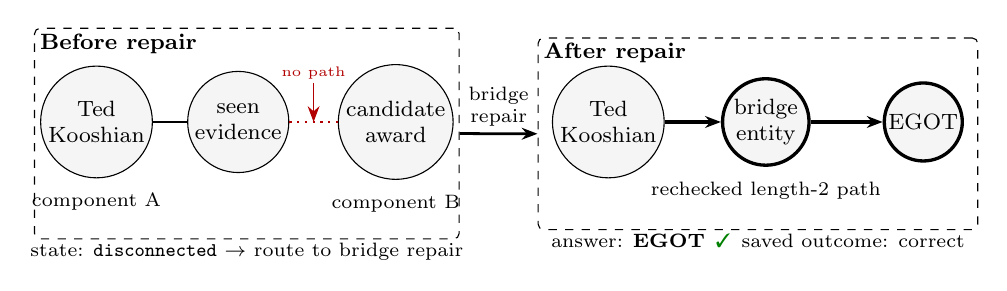
\begin{tikzpicture}[
  font=\footnotesize,
  >={Stealth[length=2mm]},
  ent/.style={draw, circle, align=center, inner sep=1pt, minimum size=8.5mm, fill=black!4},
  newent/.style={ent, very thick},
  lab/.style={font=\scriptsize, inner sep=1pt},
  panel/.style={draw, dashed, rounded corners=2pt, inner sep=5pt},
  ptitle/.style={font=\footnotesize\bfseries, anchor=north west, inner sep=2pt}
]

% ================= BEFORE =================
\node[ent] (ted) at (0,0) {Ted\\Kooshian};
\node[ent] (ev)  at (1.8,0) {seen\\evidence};
\node[ent] (award) at (3.8,0) {candidate\\award};
\draw[-] (ted) -- (ev);
\draw[red!70!black, line width=0.8pt, dotted] (ev) -- (award)
  coordinate[pos=0.5] (np);
\node[lab, red!70!black, font=\tiny, above=5mm of np] (npl) {no path};
\draw[red!70!black, ->, line width=0.4pt] (npl.south) -- (np);

\node[lab, below=1.5mm of ted]   {component A};
\node[lab, below=1.5mm of award] {component B};

\begin{scope}[on background layer]
\node[panel, fit=(ted)(ev)(award)(npl), inner sep=2pt, yshift=-1.5mm, inner ysep=6mm] (before) {};
\end{scope}
\node[ptitle] at (before.north west) {Before repair};
\node[lab, anchor=north] at (before.south)
  {state: \texttt{disconnected} $\rightarrow$ route to bridge repair};

% ================= AFTER =================
\node[ent]    (ted2)   at (6.5,0)  {Ted\\Kooshian};
\node[newent] (bridge) at (8.5,0)  {bridge\\entity};
\node[newent] (egot)   at (10.5,0) {EGOT};
\draw[->, very thick] (ted2) -- (bridge);
\draw[->, very thick] (bridge) -- (egot);
\node[lab, below=1.5mm of bridge] {rechecked length-2 path};

\begin{scope}[on background layer]
\node[panel, fit=(ted2)(bridge)(egot), yshift=-1.5mm, inner ysep=5mm] (after) {};
\end{scope}
\node[ptitle] at (after.north west) {After repair};
\node[lab, anchor=north] at (after.south)
  {answer: \textbf{EGOT}\enspace\textcolor{green!50!black}{\ding{51}}\enspace saved outcome: correct};

% ================= transition arrow =================
\draw[->, line width=1pt]
  (before.east) -- node[lab, above=1pt, align=center] {bridge\\repair} (after.west);

\end{tikzpicture}
\caption{Replayable Repair Trace for a representative saved case. The
question, graph state, repair, reader route, and answer are all recoverable
from saved fields, so the before/after repair decision can be audited without
regeneration.}
\label{fig:repair_trace_case}
\end{figure}

Table~\ref{tab:ablations} reports four operational removals on both datasets.
Two switches are intentionally compound: disabling structural checking also
disables gap-driven repair, and disabling reader context also disables
passage-based answer refinement. The largest answer-quality drop comes from
removing reader-context and refinement, which reduces HotpotQA EM from 0.5620 to
0.2360 and 2Wiki EM from 0.6900 to 0.1840. This result shows that graph triples
alone do not provide enough surface evidence for robust answer realization.

The checker removal should be read as loss of evidence-state observability, not
as an isolated EM ablation. When chain checking and repair are disabled, the
reader can still answer from unchecked context, so answer-level effects are
mixed and HotpotQA even increases slightly. The 0.6-point EM difference between
the full protocol and the no-checker variant is not statistically distinguishable
(exact McNemar $p=0.659$ over 1000 paired examples). The operational loss is
clearer: the system no longer records whether the reader saw a checked path,
repaired path, residual graph gap, or fallback evidence, and it loses the typed
state needed to route graph repair versus reader inspection.

\begin{table}[!htbp]
\centering
\caption{Compound operational removals for \sys. Full rows use the
selector-variant protocol; ablations use explicit switches, with two compound
rows labeled in the text rather than interpreted as isolated causal effects.}
\label{tab:ablations}
\small
\setlength{\tabcolsep}{4.0pt}
\begin{tabular}{lrrrr}
\toprule
\multirow{2}{*}{Variant} & \multicolumn{2}{c}{HotpotQA-1000} & \multicolumn{2}{c}{2Wiki-500} \\
\cmidrule(lr){2-3}\cmidrule(lr){4-5}
 & EM & F1 & EM & F1 \\
\midrule
Full \sys selector protocol & 0.5620 & 0.6564 & 0.6900 & 0.7581 \\
w/o state checker + repair & 0.5680 & 0.6647 & 0.6780 & 0.7579 \\
w/o graph repair & 0.5540 & 0.6580 & 0.6500 & 0.7424 \\
w/o reader context + refinement & 0.2360 & 0.2899 & 0.1840 & 0.2289 \\
w/o answer refinement & 0.5510 & 0.6485 & 0.6900 & 0.7782 \\
\bottomrule
\end{tabular}
\end{table}

\subsection{QA Quality Preservation}

The final result is an answer-quality preservation boundary. On HotpotQA-1000,
the saved \sys end-to-end row reaches 55.0\% EM / 64.8\% F1 and the deterministic
selector-sensitivity row reaches 56.2\% EM / 65.6\% F1, within the operating
range of HopRAG strict (54.1\% / 64.4\%) and A-RAG (51.7\% / 62.7\%). Paired
full-set intervals against HopRAG cross zero (selector $\Delta$EM 0.021, 95\%
CI $[-0.008,0.050]$), so these rows are not a new SOTA claim; the systems claim
rests on the added state trace, replay, and routing utility. The HotpotQA bridge
subset remains exploratory but positive ($\Delta$EM 0.058, 95\% CI
$[0.016,0.100]$).

On 2WikiMultiHopQA-500, the context-rich reader-full audit row reaches 69.0\%
EM / 75.8\% F1, near LightRAG (67.4\% / 77.2\%) and A-RAG (66.6\% / 73.2\%);
the local-context stress row reaches 50.4\% / 59.5\% and marks the stricter
context boundary. Reader-full \sys is positive against HopRAG ($\Delta$EM
0.126, 95\% CI $[0.084,0.166]$) but not separated from LightRAG or A-RAG,
confirming that context budget must be reported explicitly.

\subsection{Retrieval-Noise Probe}

Under live Web retrieval (Tavily API, 100 HotpotQA questions, seed=123,
top-5 snippets, pipeline unchanged), the state distribution shifts sharply:
checked-path rates drop from 29.0\% to 20.0\%, repaired-path rates drop from
31.0\% to 13.0\%, and residual-gap rates rise from 39.0\% to 67.0\%; the
single benchmark fallback row (1.0\%) becomes checked under live retrieval.
Of the 29 benchmark-checked questions, 17 degrade to residual and 3 trigger
successful bridge repair; of the 31 benchmark-repaired questions, 17 degrade
to residual but 8 remain repaired. The degradation and the survival of the
repair route confirm that the state contract correctly responds to retrieval
noise. The probe is exploratory (N=100), tests state-contract behavior not
answer quality, and is replayable from archived search results.

% ============================================================
\section{Discussion}
\label{sec:discussion}
% ============================================================

The main implication is that GraphRAG systems need observability, not only
better retrieval and generation. Databases expose transaction logs, and
distributed systems expose traces; fixed-context Web Knowledge-RAG similarly
needs an evidence-state trace that records what graph condition the reader saw
before an answer was produced. \sys supplies such a trace for four operational
states: checked path, repaired path, residual gap, and passage fallback.

\paragraph{Why replayability matters.}
Traditional logs record what happened, but replayable evidence-state traces also
allow operators to reconstruct why a routing decision was made and independently
verify audit conclusions without regenerating answers. This distinction matters
for production GraphRAG because repeated execution may no longer be identical
after model, prompt, index, or Web-context changes. By storing the pre-reader
state, repair route, fallback tag, and selection decision, \sys turns failure
analysis from passive log inspection into reproducible post-deployment audit.

The evidence-state trace is most valuable for failure attribution. A wrong
answer with a checked path should first be inspected as a reader or selector
failure. A wrong answer with a residual gap should first be inspected as graph
construction or bridge-repair failure. A fallback case should be inspected as a
retrieval or context-visibility failure. This routing story also explains the
mixed ablations: removing the checker does not have to reduce EM if the reader
can still answer from unchecked text, but it removes the state needed to decide
which subsystem should be repaired.

The state labels should not be read as semantic proof that the evidence is
sufficient. The 2Wiki gold-chain and blind audits show that structural labels
only partially align with human or gold-proxy notions of support. This is a
feature of the claim boundary: \sys makes evidence state visible and replayable;
it does not replace semantic verification, professional adjudication, or
uniform-budget Web retrieval.

\sys's contribution is orthogonal to retrieval and generation quality: it
neither significantly improves nor degrades the answer-quality operating range
and should be evaluated as an observability layer, not as a replacement for the
reader or retriever, the same way a tracing system is not judged by whether it
speeds up the traced service.

% ============================================================
\section{Threats to Validity}
\label{sec:limitations}
% ============================================================

\paragraph{Protocol validity.}
The experiments define a fixed-context Web Knowledge-RAG setting with recorded,
but not uniform, context budgets. Our experiments support graph-state visibility
under fixed-context Web QA settings: every reported row has a saved evidence
condition, the 2Wiki table separates reader-full and local-context rows, and the
verifier recomputes the main claims without fresh generation. Section~5.5 provides only a small-sample retrieval-noise probe; deployment-scale
evaluation under open-domain retrieval and dynamic Web environments remains
future work.

\paragraph{Diagnostic validity.}
The checker is structural rather than semantic, depends on lexical mapping and
coarse answer-type filters, and only partially aligns with gold 2Wiki paths. The
gold-chain, proxy, and blind audits calibrate the saved states as
routing metadata while keeping semantic evidence validation separate.

\paragraph{Deployment validity.}
The artifact boundary has practical consequences: 2Wiki lacks a completed MS
GraphRAG run, ablations are partly compound, and the selector row is
deterministic postprocessing. Passage fallback remains lightly exercised:
5/1000 HotpotQA and 0/500 2Wiki benchmark rows, and the retrieval-noise probe
of Section~5.5 also does not trigger it, since Web search rarely returns
unusable text for these questions; the fallback route is therefore preserved
in the state contract and verifier but not stress-tested. Future work should
add professional gap-label adjudication, fallback stress tests, semantic
repair-success analysis, and deployment-scale uniform-budget Web retrieval
runs.

% ============================================================
\section{Conclusion}
\label{sec:conclusion}
% ============================================================

We presented \sys, a replayable evidence-state auditing and routing layer for
fixed-context Web Knowledge-RAG. By shifting audit logging from only the
answer string to the retrieved evidence graph, \sys exposes checked paths,
repaired paths, residual gaps, passage fallback, and answer-selection state as
recomputable audit metadata. The result is not a claim that structural graph
state certifies correctness, but a practical evidence-state trace that may help
operators replay, inspect, and analyze GraphRAG failures after deployment.

\begingroup
\tiny
\setlength{\itemsep}{0pt}
\setlength{\parsep}{0pt}
\setlength{\parskip}{0pt}
\bibliographystyle{splncs04}
\bibliography{comagraag}
\endgroup

\end{document}
